\chapter{Architettura del sistema}
\label{chap:architettura}

\section{Modello di rete}
\label{sec:modello_rete}
Il modello di rete utilizzato è quello del \acf{RGG}, una rete di nodi rappresentata da un grafo connesso. I nodi sono connessi tra loro utilizzando il criterio di distanza geometrica, quindi ogni nodo sarà collegato con tutti quei nodi che sono ad una distanza uguale o inferiore al raggio $\rho$ da esso. Il raggio $\rho$ sarà una variabile del nostro problema. \medskip

\noindent{La generazione della rete dipende da:}
\begin{itemize}
	\item Densità dei nodi.
	\item Numero di nodi che compongono la rete.
	\item Raggio d'azione del \acs{BLE} (\textit{$\rho$}).
\end{itemize}
La scelta di operare a diversi livelli di densità è dovuta al fatto di voler studiare il comportamento della nostra soluzione in alcuni scenari urbani possibili per diverse distribuzioni geografiche sul territorio. In altre parole poter studiare il variare del comportamento del nostro algoritmo sia in situazioni di centri urbani molto densamente popolati, ad esempio medie/grandi città, sia in centri urbani con una più bassa concentrazione urbana che rappresentano la maggioranza dei paesi italiani.
Per queste considerazioni, abbiamo ipotizzato di associare al singolo nodo un abitante, come riportato dall'indagine ISTAT \cite{istat2014}. Abbiamo scelto come prima e più grande densità $ d=0.02\,nodi/m^2$ perché ci è sembrato una densità già sufficientemente alta per avere ottimi valori in termini di prestazioni, quindi scegliere densità superiori non ci è sembrato utile per il nostro scopo; inoltre questo valore è simile al valore della densità degli abitanti di Roma. Quello che invece abbiamo voluto studiare è come si degradano le prestazioni al diradarsi della concentrazione urbana, ed ecco il perché della scelta delle alte densità. In \myFig{fig:rgg_gen_02} è riportato un esempio di RGG di $ N=50 nodi$, con densità $ d=0.0005\,nodi/m^2$ e raggio $ \rho=50\,m $. Come discuteremo più avanti, possiamo notare come la scelta di una bassa densità porti alla formazione di sottoreti e all'isolamento di alcuni nodi.
\medskip

%\begin{figure}[t]
%	\subfloat[RGG con $ N=50 $, $ d=0.0005 \, nodi/m^2$ e $ \rho=50\,m$.\label{subfig-1:rgg_gen_02}]{%
%		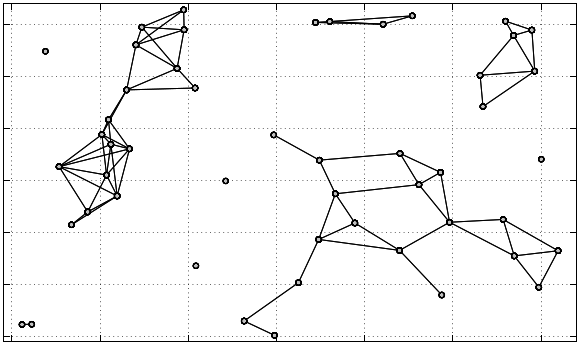
\includegraphics[width=0.60\textwidth, keepaspectratio]{Images/reti/RandomGeometricGraph_15}
%	}
%	\hfill
%	\subfloat[RGG su Tkenv.\label{subfig-2:rgg_06}]{%
%		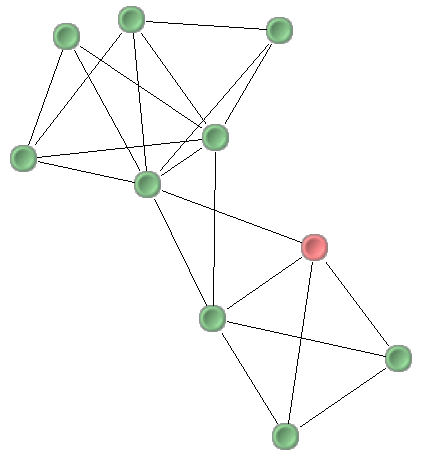
\includegraphics[width=0.30\textwidth, keepaspectratio]{Images/reti/RandomGeometricGraph_06}
%	}
%	\caption{Esempi di Random Geometric Graph.}
%	\label{fig:rgg_gen_02}
%\end{figure}
\begin{figure}[t]
	\centering
	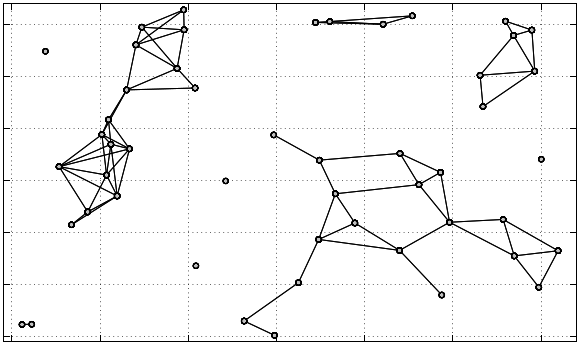
\includegraphics[width=0.8\textwidth, keepaspectratio]{Images/reti/RandomGeometricGraph_15}
	\caption[RGG con configurazione]{RGG con $ N=50 $, $ d=0.0005 \, nodi/m^2$ e $ \rho=50\,m$.}
	\label{fig:rgg_gen_02}
\end{figure}

\noindent{Le densità scelte sono:}
\begin{itemize}
	\item d = 0.02 $ \dfrac{nodi}{m^{2}} $.
	\item d = 0.01 $ \dfrac{nodi}{m^{2}} $.
	\item d = 0.008 $ \dfrac{nodi}{m^{2}} $.
	\item d = 0.001 $ \dfrac{nodi}{m^{2}} $.
	\item d = 0.0005 $ \dfrac{nodi}{m^{2}} $.
	\item d = 0.0001 $ \dfrac{nodi}{m^{2}} $.
\end{itemize}
Come già detto, abbiamo scelto di prendere come massima densità quella di Roma e poi abbiamo scelto altri valori sempre più piccoli. Per poter far riferimento ad altre situazioni reali, abbiamo scelto anche la densità della città di Milano $ d=0.008\,nodi/m^2 $. Poi abbiamo scelto valori sempre più piccoli fino a rappresentare il generico piccolo paese di campagna.

La generazione dell'area dipende anche dal numero di nodi, in quanto per mantenere un certo valore di densità è necessario che il rapporto tra il numero di utenti e l'area analizzata sia corretto. Quindi per ogni densità abbiamo scelto di fare molteplici prove con diversi valori di utenti. I valori di N che vanno da 2 a 100, sono valori pensati per simulare situazioni reali, mentre i valori più grandi sono stati scelti per vedere la scalabilità della nostra soluzione e poter studiare come si comporta il sistema in situazioni limite.
\medskip

\noindent{I valori per il numero di nodi scelti sono:}
\begin{itemize}
	\item $ N = 2 $.
	\item $ N = 5 $.
	\item $ N = 10 $.
	\item $ N = 30 $.
	\item $ N = 50 $.
	\item $ N = 80 $.
	\item $ N = 100 $.
	\item $ N = 200 $.
	\item $ N = 500 $.
	\item $ N = 1000 $.
\end{itemize}
Come già anticipato, una volta fissata la densità e il numero di nodi si ricavano le misure dell'area in analisi. Abbiamo scelto di operare in questo modo perché scegliere direttamente la grandezza dell'area senza vincoli, avrebbe portato alla scelta di aree troppo piccole o troppo grandi. Un area troppo piccola per il numero di nodi scelto, ha come conseguenza di presentare prestazioni perfette sempre, mentre scegliere un'area troppo grande restituirebbe la non utilità del sistema, a causa della troppa dispersione spaziale dei nodi. Scenari di questo tipo non sono oggetto delle nostre analisi.

Infine l'ultimo parametro che abbiamo voluto far variare è stato il raggio d'azione $\rho$ del \acs{BLE}. Le specifiche tecniche non danno nessuna indicazione della distanza coperta da questa tecnologia, perché, rispetto al precedente BT Classic, la scelta di questo fattore viene delegato alle aziende produttrici dei trasmettitori. La distanza dipende da quanto potente viene costruito un trasmettitore.
Lo studio \cite{tesi_tibertoa2013} ha stimato che in media la distanza è di 50 m, ma altri studi hanno rilevato che si può arrivare anche ad oltre 100 m in linea d'aria. Per il nostro caso di studi, poiché i dispositivi in analisi sono dispositivi mobili come smarthphone e tablet, abbiamo scelto di prendere un valore pessimistico e uno ottimistico. Questo perché, i trasmettitori equipaggiati sui dispositivi mobili non sono tutti uguali e quindi la scelta di studiare due valori agli estremi ci è parsa logica.
\bigskip\bigskip

\noindent{I valori di $ \rho $ scelti sono:}
\begin{itemize}
	\item $\rho = 15 m$.
	\item $\rho = 50 m$.
\end{itemize}
Abbiamo scelto di utilizzare come valore più piccolo, un raggio poco più grande di quello della Classe 2 del Bluetooth Classic, che è di norma la distanza raggiunta dai dispositivi cellulari precedenti gli smartphone. Come termine massimo invece, abbiamo scelto di utilizzare il valore medio stimato dallo studio \cite{tesi_tibertoa2013}. Ci è sembrato sensato che un normale smartphone non vada oltre i 50 m per un motivo: gli smartphone e i tablet sono soggetti ad una progettazione minimalista che cerca di compattare il più possibile in pochi millimetri di spessore. Questo comporta ad installare trasmettitori di potenza sufficiente per coprire l'utilizzo di componenti accessori come i dispositivi wearable e che possano occupare lo spazio desiderato dai designer, a differenza dei trasmettitori progettati per applicazioni in ambito industriale, i quali devono coprire a volte distanze anche superiori a 100 m e vengono progettati con l'obiettivo primario della distanza, senza vincoli di volume.

\subsection{Costruzione della rete}
In fase di simulazione, la generazione della rete viene fatta in modo automatico dal simulatore come la distribuzione dei nodi nell'area e la costruzione dei collegamenti tra i nodi. I vari parametri necessari, grandezza dell'area, numero dei nodi e raggio $\rho$ sono inseriti negli appositi file d'inizializzazione. Quando viene eseguito lo script di lancio, viene caricato il file di inizializzazione corrispondente al caso di simulazione e nel file di Network Definition vengono caricati i valori dei parametri specificati nel file di inizializzazione caricato. Il file \acs{NED} relativo al \acs{RGG}, si veda ad esempio il codice all'\MyAppendix{fig:rgg_code}, contiene i metodi per la costruzione della rete. Come prima cosa, i nodi vengono posizionati in maniera casuale e uniforme nell'area specificata, poi nella sezione \textit{connections} vi è il metodo che controlla e inserisce i collegamenti tra i nodi. Dopo aver disposto casualmente i nodi nell'area, per ogni nodo controlla quali altri nodi si trovano ad una distanza geometrica inferiore al valore di $\rho$ specificato nel file di inizializzazione e tra essi inserisce un canale di comunicazione con le prestazioni di trasmissione del \acs{BLE} (Velocità di trasmissione $ 1Mbps $ e ritardo di $ 3ms $).

\section{Algoritmo Dynamic Fanout}
\label{sec:alg_df}
Come presentato nella \MySec{chap:Prog_log_sol} la nostra soluzione è una estensione dell'algoritmo di gossip Fixed Fanout (vedere \MySec{subsec:alg_p2p}). Abbiamo esteso il metodo di calcolo per il limite del numero di trasmissioni che ogni nodo può effettuare, inserendo nuove componenti dinamiche che hanno reso lo stesso fattore reattivo ai cambiamenti sia ambientali sia interni al dispositivo. Per questo motivo abbiamo chiamato il nostro algoritmo: Dynamic Fanout. Successivamente, abbiamo aggiunto un controllo per la terminazione delle trasmissioni che risultano essere inutili, permettendo all'algoritmo di limitare gli sprechi di energia. In questo modo il sistema cerca sempre di trovare un punto di lavoro che offra un compromesso tra efficienza e risparmio energetico nella maggior parte degli scenari studiati.

I due principali fattori che abbiamo progettato sono il Dynamic Fanout e l'Advertising Limit. Questi parametri sono due criteri di terminazione di tipo \textit{counter}, ma che al loro interno hanno anche una componente di tipo \textit{blind} necessaria a valutare lo stato della batteria del dispositivo. Il Dynamic Fanout rappresenta il limite di trasmissioni che il dispositivo può fare nel suo stato, mentre l'Advertising Limit rappresenta il limite di trasmissioni di advertising andate a vuoto consecutivamente che il dispositivo deve fare prima di decidere che nessuno dei suoi vicini è più interessato all'informazione che possiede.

Il nostro algoritmo agisce basandosi sulla macchina a stati del \acs{BLE}, cambiando stato all'avvenire di particolari eventi. Avendo fatto una relazione uno a uno tra gli stati dell'algoritmo di gossip e quelli della macchina a stati del \acs{BLE}, abbiamo potuto centralizzare la gestione sul Bluetooth. Anche se il \acs{BLE} per definizione è un sistema di trasmissione che consuma poca energia, abbiamo deciso che il nostro sistema sia in uno stato di attiva operatività finché la batteria del dispositivo è superiore al 10\%. Questo perché, non vogliamo che il sistema vada a consumare le ultime riserve di energia del dispositivo, permettendo all'utente di usufruire di tutti quei servizi di cui ha bisogno e di raggiungere eventualmente una fonte di ricarica. Inoltre la maggior parte degli smartphone implementa già sistemi di risparmio energetico che disabilitano i sistemi non essenziali quando la batteria scende sotto certi livelli.
Il nostro algoritmo, qualora la batteria scenda sotto il 10\%, finisce l'eventuale trasmissione in corso e poi si porta in stato di Standby. Quando la batteria torna sopra il 10\%, il sistema torna attivo e operativo. Questo controllo viene fatto periodicamente, tramite una procedura che esegue le "azioni periodiche". Sono azioni che devono essere eseguite ciclicamente, indipendentemente dall'occorrenza di eventi esterni. Queste azioni periodiche prevedono il controllo dello stato della batteria e l'aggiornamento dei parametri. Questo processo rimane attivo anche quando la batteria scende sotto la soglia limite e continua i suoi aggiornamenti, così da poter riattivare subito il sistema quando la batteria viene caricata. Nel nostro caso di studio abbiamo simulato la decadenza della batteria tramite il decremento di una variabile numerica.
\begin{algorithm}[t]
	\caption{Azioni Periodiche}\label{alg:periodic_actions}
	\begin{algorithmic}[1]
		\Function{AzioniPeriodiche}{\textit{btState}}
		\State \textit{decrementaBatteriaIdle()}
		\State $ \textit{batteria} \gets \textit{livelloBatteria() } $
		\If{$\left(  \textit{busy} \: || \: \textit{batteria} \geq 0 \right) $}
		\State \textit{AggiornaParametri(\textit{batteria})}
		\If{$\textit{btState} = STANDBY $}
		\State $ \textit{btState} \gets INITIATING $
		\EndIf
		\Else
		\State $ \textit{btState} \gets STANDBY $
		\EndIf
		\EndFunction
	\end{algorithmic}
\end{algorithm}
Un decremento costante ad ogni azione periodica per simulare il normale consumo della batteria, più un consumo ad ogni trasmissione/ricezione che il dispositivo effettua, per accentuare il fatto che il consumo energetico del sistema è concentrato nelle trasmissioni e non nel suo stato di attesa. Abbiamo scelto di decrementare la batteria ad ogni azione periodica, col risultato di un consumo energetico medio più alto di quello reale dovuto al solo \acs{BLE}, per studiare come si comporta il sistema in quei dispositivi soggetti ad un alto consumo energetico medio proprio. Lo pseudo codice dell'\MyAlg{alg:periodic_actions} descrive il funzionamento delle azioni periodiche, che vengono schedulate periodicamente dal sistema.
\begin{algorithm}[ph]
	\caption{Invio Messaggio}\label{alg:invia_msg}
	\begin{algorithmic}[1]
		\Function{InvioMessaggio}{\textit{btState},\textit{msg}}
		\If{$\textit{btSt}ate \neq STANDBY$}
		\State $ \textit{btState} \gets STANDBY$
		\EndIf
		\State $ \textit{Tx counter} \gets 0 $ \Comment{Contatore trasmissioni effettuate.}
		\Label \spacedlowsmallcaps{start:}
		\State $ \textit{AE counter} \gets 0 $ \Comment{Contatore degli Advertising Event.}
		\State $ \textit{btState} \gets ADVERTISING$
		\State $ AE counter \gets +1 $
		\State \textbf{begin}
		\State\hspace{\algorithmicindent}{ADVERTISING EVENT}
		\State \textbf{end}
		\If{$\textit{èTimeoutScaduto()}$}
		\If{$ \textit{AE counter}\,<\,\textit{AL}$}\Comment{AL = Advertising Limit.}
		\State \textbf{go to} \spacedlowsmallcaps{start}
		\Else
		\State $btState \gets STANDBY$
		\State \textit{AzioniPeriodiche(btState)}
		\EndIf
		\EndIf
		\State $ \textit{busy}\gets VERO $
		\State $\textit{btState}\gets CONNECTION\_SLAVE$
		\State \textbf{begin}
		\State\hspace{\algorithmicindent}{CONNECTION EVENT}
		\State \textbf{end}
		\State $\textit{Tx counter}\gets +1$
		\State $ \textit{decrementaBatteriaTx()}$
		\State $\textit{busy}\gets FALSO$
		\State $ \textit{btState}\gets STANDBY $
		\If{$ \textit{Tx counter}\,<\,DF$}
		\State \textbf{go to} \spacedlowsmallcaps{start}
		\Else
		\State \textit{AzioniPeriodiche(btState)}
		\EndIf
		\EndFunction
	\end{algorithmic}
\end{algorithm}
La variabile booleana \textit{busy} segnala quando il dispositivo è impegnato nell'esecuzione di qualche trasmissione o ricezione. All'\MyAppendix{apx:stb_fsa}, riportiamo il diagramma di flusso della macchina a stati Standby. Questo diagramma sintetizza il comportamento del sistema nei momenti di inattività. All'avvenire di azioni periodiche, il sistema controlla il livello di batteria e se maggiore del 10\%, porta il sistema in stato di Initiating. Se il sistema riceve dall'utente il comando di inviare un messaggio, esso passa in modalità di invio di un nuovo messaggio e l'\MyAlg{alg:invia_msg} descrive in pseudo codice le operazioni necessarie all'invio di dati.

All'\MyAppendix{apx:invio_fsa} riportiamo il diagramma di flusso della macchina a stati dell'\MyAlg{alg:invia_msg}. Per inviare un messaggio, il sistema entra si porta in stato di Standby se non lo fosse già stato, inizializza le variabili contatore per il numero di trasmissioni e per gli \acf{AE} e poi e passa in stato di Advertising. A questo punto incrementa il contatore degli \acs{AE} e inizia l'\acs{AE} vero e proprio. Dopo aver trasmetto i suoi pacchetti, si mette in attesa di una risposta. Se il timeout scatta prima che una richiesta di connessione arrivi, allora quell'\acs{AE} viene considerato a vuoto. Viene incrementato il relativo contatore, quindi controllato che il numero di \acs{AE} a vuoto non sia superiore all'\acs{AL}; se il limite non è raggiunto, si ricomincia con un altro \acs{AE}. Se invece il contatore di \acs{AE} è maggiore o uguale dell'\acs{AL}, il sistema si ferma e si riporta sulle azioni periodiche e quindi in stato di ascolto (Initiating). Se invece, prima che scada il timeout, riceve una richiesta di connessione, allora il sistema si dichiara \textit{busy}, occupato, si porta nello stato di Connection col ruolo di Slave e attende che il \acf{CE} cominci. Una volta terminata la trasmissione, incrementa il contatore delle trasmissioni, resetta il contatore degli \acs{AE}, si dichiara non più occupato e si porta in stato di Standby. Infine il sistema controlla se ha effettuato \acs{DF} transazioni. In caso negativo si riporta all'inizio di tutta la procedura di invio, in caso positivo esce e riprende le azioni periodiche riportandosi in stato di ascolto.

Se il sistema rileva la presenza di un nuovo messaggio sulla rete, esso passa in modalità di ricezione di un nuovo messaggio e l'\MyAlg{alg:ricevi_msg} descrive in pseudo codice le operazioni necessarie. All'\MyAppendix{apx:ricevi_fsa} riportiamo il diagramma di flusso della relativa macchina a stati. Il fatto di rilevare un informazione nuova presuppone che il sistema sia in stato di Initiating. Se il sistema sta nello stato di Initiating, automaticamente resta in ascolto di nuove informazioni. Una volta nello stato di ascolto, quando rileva una nuova informazione, il sistema manda una richiesta di connessione al mittente del pacchetto di advertising. Dopo di che si segna come occupato ed entra nello stato di Connection col ruolo di Master e invia la richiesta di apertura del Connection Event. Se il timeout scade, vuol dire che la richiesta di connessione non è stata accettata e quindi il sistema si dichiara non più occupato e si riporta in stato di ascolto. Se invece la richiesta di connessione viene accetta, alla richiesta di apertura del Connection Event segue in risposta l'informazione, così da entrare definitivamente nel Connection Event. Completata la ricezione del messaggio, esso viene salvato, il sistema si dichiara non occupato e poi inizia ad inviare a sua volta questo nuovo messaggio.
\begin{algorithm}[t]
	\caption{Ricevi Messaggio}\label{alg:ricevi_msg}
	\begin{algorithmic}[1]
		\Function{RiceviMessaggio}{\textit{btState}}
		\If{$\textit{btState = INITIATING}$}
			\State \textbf{go to} \spacedlowsmallcaps{send}
		\EndIf
		\Label \spacedlowsmallcaps{start:}
		\State $\textit{btState} \gets STANDBY$
		\State $\textit{btState} \gets INITIATING$
		\Label \spacedlowsmallcaps{send:}
		\State $ \textit{invioRichiestaConnessione()}$
		\State $ \textit{busy} \gets VERO$
		\State $ \textit{btState} \gets CONNECTION\_MASTER $
		\State $ \textit{inviaRichiestaPool()}$\Comment{Richiesta d'apertura di C.E.}
		\If{$\textit{èTimeoutScaduto()}$}
			\State $ \textit{busy} \gets FALSO$ \Comment{La richiesta non è stata accettata.}
			\State \textbf{go to} \spacedlowsmallcaps{start}
		\EndIf
		\State \textbf{begin}
			\State\hspace{\algorithmicindent}{$\textit{msg} \gets CONNECTION EVENT$}
		\State \textbf{end}
		\State $ \textit{decrementaBatteriaTx()} $
		\State $ \textit{busy} \gets FALSO$
		\State $ \textit{InvioMessaggio}\left(\textit{msg,btState}\right)  $
		\EndFunction
	\end{algorithmic}
\end{algorithm}

\subsection{\acf{DF}}
Il Dynamic Fanout ha il compito di fermare il dispositivo dopo un certo numero di trasmissioni effettuate con successo per una certa informazione. Questo valore limite è calcolato in modo dinamico, dipendente dal livello di batteria del dispositivo e dal numero di nodi che il sistema riesce a percepire, quindi al numero di nodi ai quali può potenzialmente connettersi. Abbiamo voluto che questo parametro avesse un particolare andamento e rapidità di risposta in particolari situazioni e altri andamenti per altre situazioni. A tale scopo, abbiamo provato a caratterizzare il comportamento di questo parametro attraverso diversi modelli matematici, ottenendo quindi comportamenti più o meno conservativi, secondo la funzione scelta.

Il calcolo del \acs{DF} è composto da due fattori: un primo fattore che tiene conto del livello di batteria del dispositivo, chiamato \textit{Fattore Batteria} e da un secondo fattore dipendente dal numero di nodi, che ha la funzione di correggere l'andamento globale della funzione risultante. La nostra idea è di ottenere dal Fattore Batteria una percentuale che rappresenta la quantità di nodi, tra quelli percepiti, che il dispositivo prenderà in considerazione come suo limite di trasmissione cioè come suo \acs{DF}. Più batteria un dispositivo ha più alta sarà la percentuale di nodi cui potremo trasmettere l'informazione. In \myFig{fig:DF_battery_factor} riportiamo in grafico tre funzioni batteria studiate, ognuna con un andamento diverso; esse sono rispettivamente:
\begin{equation}
	\label{eq:df_bat_radq}
	y=\dfrac{\sqrt{0,2\cdot x\,-\,1,9}}{10}
\end{equation}
\begin{equation}
	\label{eq:df_bat_ln}
	y=\dfrac{\ln\left(x\,-\,8\right) }{10}
\end{equation}
\begin{equation}
	\label{eq:df_bat_log}
	y=\dfrac{\log\left(x\,-\,8\right) }{10}
\end{equation}
\begin{figure}[tb]
	\centering
	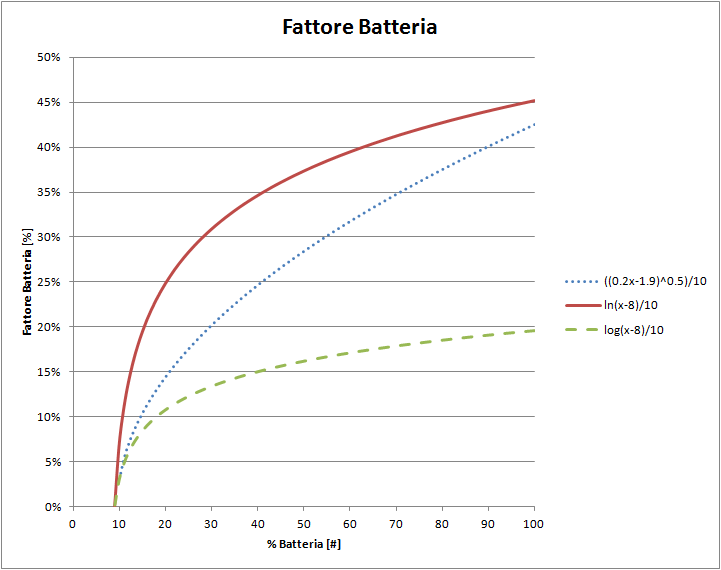
\includegraphics[width=0.9\linewidth, keepaspectratio]{Images/grafici_usati/DF_battery_factor}
	\caption[Curve Fattore Fatteria (DF).]{Curve delle Funzioni Batteria per il \acs{DF}.}
	\label{fig:DF_battery_factor}
\end{figure}
Da un punto di vista matematico la ricerca di un comportamento fortemente crescente all'inizio, con una successiva crescita più moderata, ci ha portato a valutare due principali tipi di funzioni: la funzione radice e la famiglia dei logaritmi. Regolando l'indice della radice o la base del logaritmo si possono ottenere comportamenti più o meno accentuati. Questo è il motivo della scelta delle funzioni che abbiamo presentato.
Tutte e tre le funzioni sono divise per dieci, così da ottenere un valore percentuale. Dalla \myFig{fig:DF_battery_factor} si nota come diversi tipi di funzioni diano differenti curve di risposta, più o meno conservative e/o reattive per valori tra 10\% e il 20\% di batteria. Noi abbiamo scelto di utilizzare la funzione di \MyEq{eq:df_bat_radq} rispetto alla funzione col logaritmo naturale, \MyEq{eq:df_bat_ln}, poiché non troppo aggressiva per valori bassi di batteria ma nemmeno eccessivamente conservativa e perché al crescere della percentuale di batteria le due funzioni tendono allo stesso valore massimo. L'\MyEq{eq:df_bat_log} risulta essere troppo conservativa e non scala bene con la crescita della batteria e della rete.
\medskip

\noindent{La funzione scelta per il Fattore Batteria è quindi:}
\begin{equation}
	\label{eq:df_FB}
	FB = \dfrac{\sqrt{0,2\cdot x\,-\,1,9}}{10}
\end{equation}
\begin{figure}[tb]
	\centering
	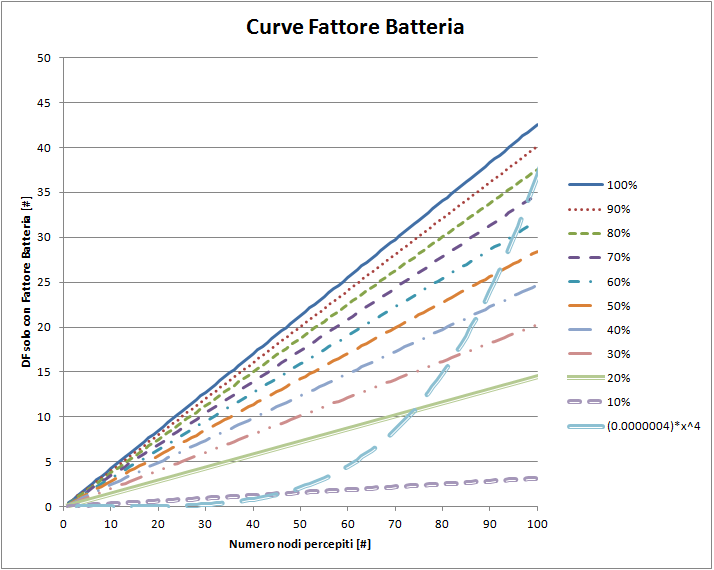
\includegraphics[width=0.9\linewidth]{Images/grafici_usati/DF_curve_fattore_batteria_corr}
	\caption[Curve Fattore Batteria con Fattore di Correzione]{Applicazione del Fattore Batteria al numero di nodi e Fattore di Correzione.}
	\label{fig:DF_curve_fattore_batteria_corr}
\end{figure}
La variabile $\textit{x}$ rappresenta la percentuale di batteria del dispositivo ed è compresa nell'intervallo [0;100]$\in\mathbb{R}$.

Il Fattore Batteria quindi indica la percentuale sulla totalità dei nodi percepiti, da utilizzare come limite di trasmissioni. L'\MyEq{eq:df_FB} restituisce un valore tra 0 e 1, che applicato al numero di nodi percepiti, genera una retta linearmente crescente, al crescere del numero dei dispositivi percepiti. In \myFig{fig:DF_curve_fattore_batteria_corr} abbiamo riportato le principali rette, una ogni 10\% di batteria. Come si può notare ogni retta è monotona crescente e ciò non va bene, perché si avrebbero limiti di trasmissioni totalmente inadeguati al crescere della rete. Abbiamo quindi pensato di introdurre un Fattore di Correzione, che aiutasse a bilanciare la crescita monotona di queste rette. Più il numero di nodi è alto, più questo fattore correttivo è forte.
\medskip

\noindent{Il Fattore di Correzione ha la seguente equazione:}
\begin{equation}
	\label{eq:df_FC}
	FC = 0.0000004x^4
\end{equation}
La variabile $\textit{x}$ rappresenta il numero di nodi percepiti dal dispositivo e $ \textit{x}\in\mathbb{N},x\geq0$. Abbiamo progettato il Fattore di Correzione in modo che possa risultare trascurabile per valori bassi di numero di nodi, mentre applichi la sua funzione correttiva per valori medio-grandi e grandi di numero di nodi. Questo è il motivo per cui abbiamo scelto un coefficiente così piccolo. In questo modo partendo da un valori piccoli, la componente dominante è il Fattore Batteria, poi al crescere dei nodi, la componente dominante diventa sempre più quella correttiva. Il motivo per cui abbiamo scelto di inserire questo Fattore di Correzione, è che ci serviva qualcosa per gestire la crescita monotona dovuta al solo Fattore Batteria e anche per scegliere meglio, con più criterio, il valore del \acs{DF}. Col crescere della rete, cresce anche la possibilità che vi siano più dispositivi nella rete con un alto livello di batteria e quindi è possibile distribuire meglio il carico di lavoro su molti più nodi. Con una rete meno densa, lasciamo che il \acs{DF} sia più grande per coprire gli eventuali dispositivi vicini che posso avere poca batteria e quindi partecipare poco o addirittura nulla al processo di diffusione. Con una rete sempre più densa invece, possiamo ridurre questo "sovraccarico", perché anche avendo la possibilità di nodi vicini con poca batteria, cresce la probabilità che vi siano altri nodi con molta batteria che possono affrontare anch'essi un buon carico di lavoro. Per questo motivo, per un alto numero di nodi, abbiamo un \acs{DF} decrescente.
Unendo quindi, Fattore Batteria e Fattore correttivo abbiamo il seguente primo calcolo del \acs{DF}.
\begin{align*}
	\label{eq:DF_no_asint}
	DF &= 1 \; + \; FB\cdot x \; - \; FC\\
	&= 1 \; + \left( \dfrac{\sqrt{0,2\cdot z\,-\,1,9}}{10}\; \right) \cdot x- \; 0.0000004x^4 \addtocounter{equation}{1}\tag{\theequation}
\end{align*}
La variabile $\textit{x}$ rappresenta il numero di nodi percepiti dal dispositivo e $ \textit{x}\in\mathbb{N},x\geq0$, mentre $\textit{z}$ rappresenta il livello di batteria e $\textit{z}\in \mathbb{R}, \textit{z}\in[0;100]$.
\begin{figure}[t]
	\centering
	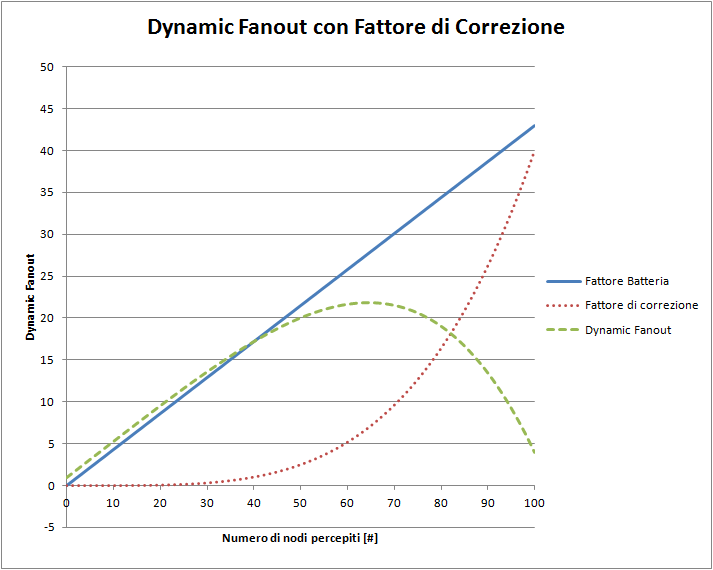
\includegraphics[width=0.9\linewidth]{Images/grafici_usati/DF_andamento_teorico}
	\caption[Andamento teorico DF]{Andamento Dynamic Fanout con correzione.}
	\label{fig:DF_andamento_teorico}
\end{figure}
In \myFig{fig:DF_andamento_teorico} è riportato su grafico la curva di questo primo calcolo di \acs{DF} con l'aggiunta del Fattore di Correzione, di uno dei possibili valori di Fattore Batteria. In questa rappresentazione grafica è stato ottenuto un \acs{DF} con un andamento crescente come il FB fino all'intorno di $\textit{x}=50\,nodi$, poi un andamento decrescente causato dall'intervento del FC. Sottolineiamo che il valore del massimo, sia in termini di valore asse $ x $ e valore asse $ y $, varia al variare del livello di batteria. Come è facile notare dal grafico, per più di 100 nodi o per curve di batteria inferiori, il \acs{DF} risulterebbe negativo. Ovviamente questo non è accettabile. Per questo motivo abbiamo anche aggiunto una componente asintotica al calcolo del \acs{DF}. L'asintoto orizzontale, è pensato per stabilizzare il \acs{DF} su di un valore, quando vi sono tanti nodi.
\begin{figure}[t]
	\centering
	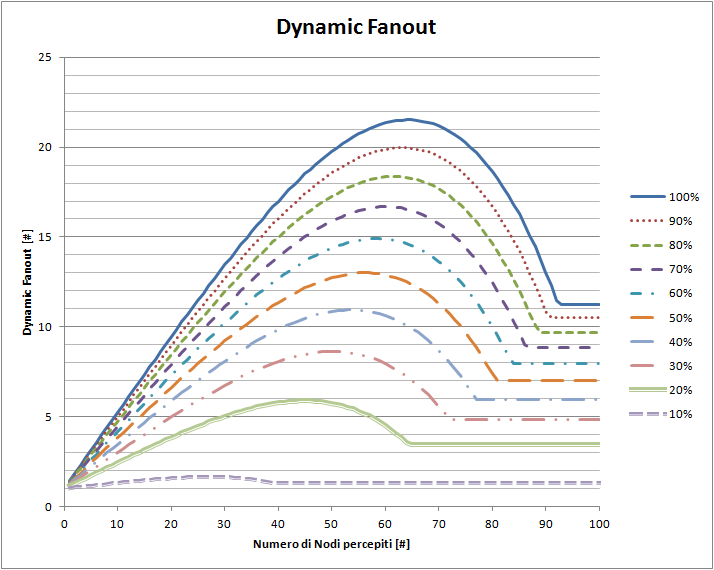
\includegraphics[width=0.9\linewidth]{Images/grafici_usati/DF_tot_no_arr}
	\caption[DF finale (continuo)]{Curve finali Dynamic Fanout.}
	\label{fig:DF_tot_no_arr}
\end{figure}
La nostra scelta è basata sull'idea che oltre un certo numero di nodi, si possa trascurare la dipendenza da essi, in quanto ci troveremmo in uno scenario di altissima densità. Quindi abbiamo pensato che è sufficiente avere un limite asintotico dipendente dal livello della batteria in modo da garantire sempre che ogni nodo non compia sforzi eccessivi consumando troppa energia. Il valore asintotico viene preso in considerazione quando il numero di nodi supera $\mathit{X_{max}}$, quel valore di \textit{x} corrispondete al $\mathit{DF_{max}}$ per quella curva. Se $\textit{x}\geq\mathit{X_{max}}$, il sistema prenderà in considerazione il valore asintotico se la curva \acs{DF} con correzione è inferiore all'asintoto. Il valore dell'asintoto è stato scelto in modo da tenere la dipendenza dal livello di batteria, così che ogni curva abbia il proprio asintoto adeguato. L'equazione dell'asintoto viene così definita:
\begin{equation}
	\label{eq:df_asintoto}
	Asintoto = 1\;+\;DF_{max}\cdot 50\%
\end{equation}
Abbiamo quindi due situazioni: $\textit{x}<\mathit{X_{max}}$ e $\textit{x}\geq \mathit{X_{max}}$. Unendo le Equazioni (\ref{eq:DF_no_asint}) e (\ref{eq:df_asintoto}) otteniamo l'\MyEq{eq:DF_totale}, equazione finale del Dynamic Fanout, rappresentato in \myFig{fig:DF_tot_no_arr}.
\begin{equation}
\scriptsize
\label{eq:DF_totale}
DF = \begin{cases} 1 + \left( \dfrac{\sqrt{0,2\cdot z - 1,9}}{10} \right) \cdot x- 0.0000004x^4 & ,\textit{x}<\textit{X}_{max}\\
					\max \left( 1 + \left( \dfrac{\sqrt{0,2\cdot z - 1,9}}{10} \right) \cdot x- 0.0000004x^4 ; 1 + \frac{1}{2}DF_{max} \right) & ,\textit{x}\geq\textit{X}_{max}\end{cases}
\normalsize
\end{equation}
\begin{figure}[t]
	\centering
	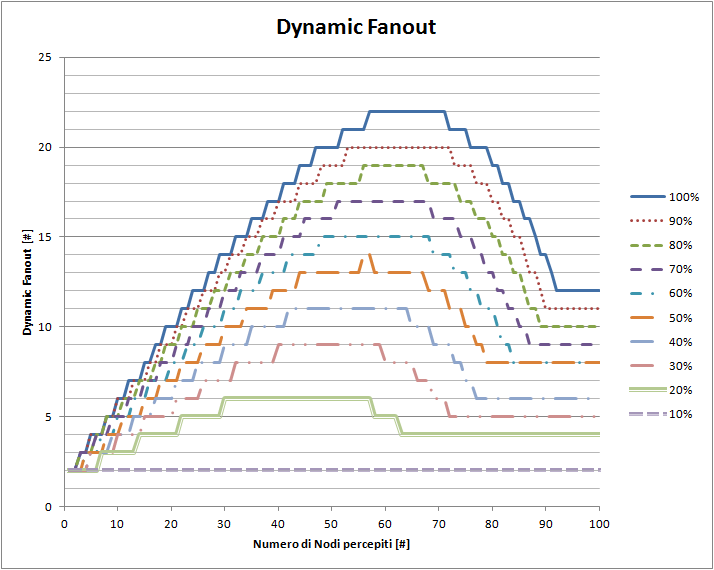
\includegraphics[width=0.9\linewidth]{Images/grafici_usati/DF_tot_arr}
	\caption[DF finale (arrotondato)]{Curve finali Dynamic Fanout, arrotondate per eccesso.}
	\label{fig:DF_tot_arr}
\end{figure}
Come prima, abbiamo rappresentato i dieci livelli di batteria. Dato che il \acs{DF} esprime il limite di trasmissioni che un nodo può fare per ogni informazione, non ha senso avere valori non interi perché il conteggio può essere fatto solo a numeri interi. Abbiamo quindi applicato un arrotondamento per eccesso alle curve mostrate in precedenza in \myFig{fig:DF_tot_no_arr}. Il risultato è riportato in \myFig{fig:DF_tot_arr}. Applicando tale arrotondamento abbiamo ottenuto un innalzamento per tutte le curve di 1; quindi avremo il valore minimo pari a 2. Questo non crea alcun problema, anzi rende il sistema ancora più permissimo per reti piccole o diradate. Al crescere del numero di nodi percepiti, questo effetto resta trascurabile. Quello riportato in \myFig{fig:DF_tot_arr} è ciò che è stato implementato nell'algoritmo.

Abbiamo studiato anche molte altre funzioni, di vario genere e con comportamenti diversi. Alcune funzioni più conservative e altre più permissive. Di seguito riportiamo solo due casi: uno più permissivo e uno più conservativo rispetto alla soluzione scelta, con le relative formule delle funzioni utilizzate. Abbiamo riportato poi, solo i grafici finali, quelli degli andamenti totali del \acs{DF} con asintoti senza arrotondamenti, per comprendere meglio le caratteristiche delle curve. Il metodo di calcolo del \acs{DF} totale è lo stesso dell'\MyEq{eq:DF_totale},  cambieranno solo le funzioni che lo compongono.
\begin{figure}[t]
	\centering
	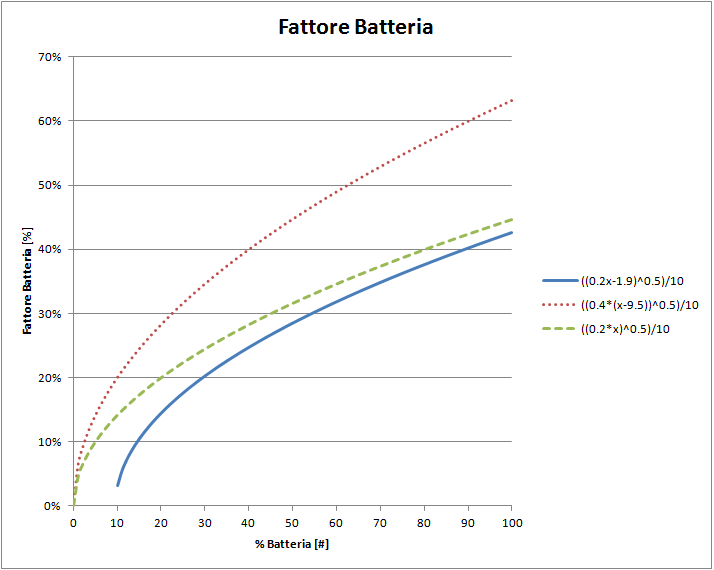
\includegraphics[width=0.9\linewidth]{Images/grafici_usati/DF_battery_factor_perm_conserv}
	\caption[Fattore Batteria alternative del DF]{Funzioni alternative per il Fattore Batteria del \acs{DF}.}
	\label{fig:DF_battery_factor_perm_conserv}
\end{figure}

Partiamo dai Fattori Batteria. Di seguito riportiamo le due funzioni in esame, più la funzione usata in soluzione, per fare meglio un confronto. Le funzioni studiate sono state molte, ma riportiamo solo quelle generate da una manipolazione della funzione utilizzata in soluzione. In \myFig{fig:DF_battery_factor_perm_conserv}, sono riportate le rispettive curve per un confronto grafico.
\begin{equation}
	\label{eq:df_bis_bat_sol}
	y=\dfrac{\sqrt{0,2\cdot x\,-\,1,9}}{10}
\end{equation}
\begin{equation}
	\label{eq:df_bis_bat_perm}
	y=\dfrac{\sqrt{0,4x}}{10}
\end{equation}
\begin{equation}
	\label{eq:df_bis_bat_cons}
	y=\dfrac{\sqrt{0,2x}}{10}
\end{equation}
L'\MyEq{eq:df_bis_bat_sol}è la stessa equazione della soluzione (\MyEq{eq:df_FB}), mentre l'\MyEq{eq:df_bis_bat_perm} e l'\MyEq{eq:df_bis_bat_cons} sono rispettivamente la funzione permissiva e la funzione conservativa.
\bigskip

\noindent{\textbf{\textit{Caso Permissivo}}}\\
Il caso permissivo, mostrato in \myFig{fig:DF_permissivo_tot_no_arr}, nasce dalla rimozione del fattore di traslazione orizzontale e dall'incremento del coefficiente della variabile \textit{x}, da 0.2 è stato alzato a 0.4. Questo gli permette di crescere più velocemente, come si può vedere in \myFig{fig:DF_battery_factor_perm_conserv}.
\medskip
\begin{figure}[t]
	\centering
	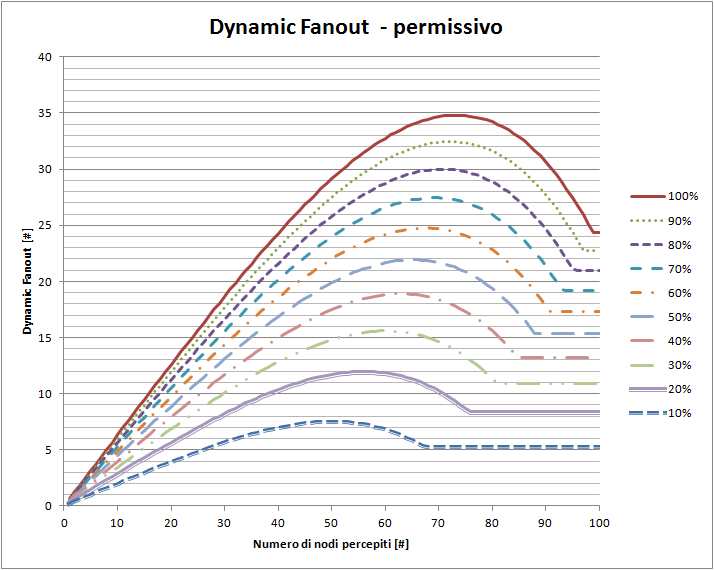
\includegraphics[width=0.9\linewidth]{Images/grafici_usati/DF_permissivo_tot_no_arr}
	\caption[Curve del DF permissivo]{Curve del \acs{DF} permissivo.}
	\label{fig:DF_permissivo_tot_no_arr}
\end{figure}

\noindent{Il Fattore Batteria quindi è:}
\begin{equation}
	FB_{perm}=\dfrac{\sqrt{0,4x}}{10}\nonumber
\end{equation}
Aumentando il coefficiente si ottiene una crescita più ripida, quindi una reattività maggiore. Avere un fattore di partizionamento molto alto può giovare alle prestazioni, ma fino ad un certo punto perché alla fine il \acs{DF} sarà così alto per ogni situazione di nodi percepiti, che tale limite non sarà mai raggiunto e quindi si userà solo l'\acs{AL} per la terminazione.
\medskip

\noindent{Il Fattore di Correzione rimane lo stesso dell'\MyEq{eq:df_FC}:}
\begin{equation}
	FC = 0.0000004x^4 \nonumber
\end{equation}
\noindent{L'asintoto invece è stato alzato al 70\% del \acs{DF} massimo:}
\begin{equation}
	\label{eq:df_asintoto_perm}
	Asintoto = DF_{max}\cdot 70\%
\end{equation}
Il calcolo del \acs{DF} rimane lo stesso della soluzione descritta in precedenza. Dal grafico si può notare che abbiamo ottenuto un incremento del valore massimo di circa 60\% o addirittura superiore, dipendente dalla curva.
\bigskip

\noindent{\textbf{\textit{Caso Conservativo}}}\\
Per il caso conservativo, presentiamo una funzione molto simile a quella utilizzata nella soluzione, l'\MyEq{eq:df_bis_bat_cons}. E' stato rimosso il fattore di traslazione, ma il coefficiente sulle \textit{x} è rimasto lo stesso. Infatti come si può vedere nel grafico in \myFig{fig:DF_battery_factor_perm_conserv}, la funzione conservativa e quella della soluzione hanno un andamento molto simile. La principale differenza di questa versione, è di avere un Fattore di Correzione più aggressivo che agisce prima, rispetto a quello usato nelle precedenti.
\begin{figure}[t]
	\centering
	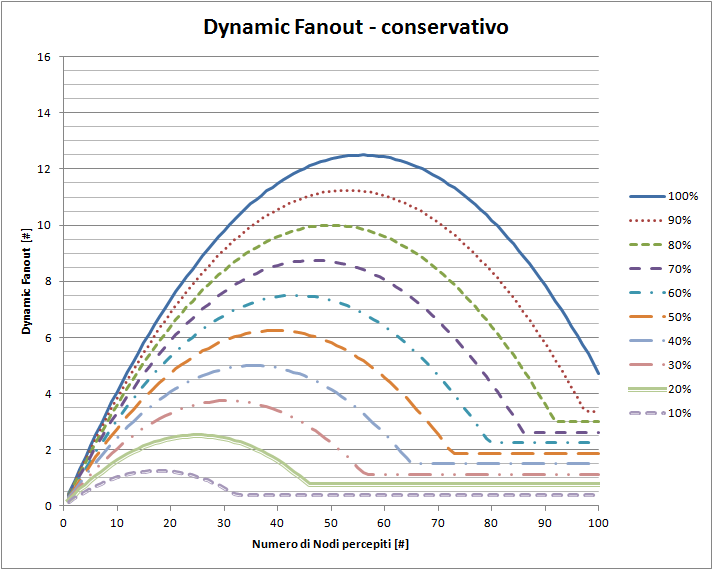
\includegraphics[width=0.9\linewidth]{Images/grafici_usati/DF_conservativo_tot_no_arr}
	\caption[Curve del DF conservativo]{Curve del \acs{DF} conservativo.}
	\label{fig:DF_conservativo_tot_no_arr}
\end{figure}
\begin{equation}
	FB_{cons}=\dfrac{\sqrt{0,2x}}{10}\nonumber
\end{equation}
Il Fattore di Correzione è cambiato, il suo coefficiente è stato aumentato e il grado della funzione diminuito, per rendere tangibile la sua correzione molto prima.
\begin{equation}
	FC = 0.004x^2
\end{equation}
Anche l'asintoto è stato cambiato e ne è stato scelto uno più basso, solo il 30\% del \acs{DF} massimo delle curve.
\begin{equation}
	Asintoto = DF_{max}\cdot 30\%
\end{equation}
Il calcolo del \acs{DF} è rimasto lo stesso di quello presentato precedentemente per la soluzione. Abbiamo riportato il risultato su grafico, in \myFig{fig:DF_conservativo_tot_no_arr}. Come si può notare dal grafico, abbiamo ottenuto una diminuzione del valore dei massimi da un 40\% a un 50\% rispetto alla soluzione implementata.
\bigskip

\subsection{\acf{AL}}
L'Advertising Limit ha il compito di segnalare al dispositivo quando smettere di pubblicizzare un'informazione, perché molto probabilmente è inutile e solo uno spreco di energia.  Durante la fase di advertising, vengono conteggiati gli \acf{AE} che vanno a vuoto, ovvero che non ricevono risposta. Se questo numero di advertising consecutivi senza successo diventa uguale o maggiore dell'\acs{AL}, significa che con molta probabilità nessuno dei nodi vicini all'advertiser è interessato a quella informazione. A causa dei tempi di attesa imposti dalla tecnologia di trasmissione, non si può avere una certezza matematica, ma avendo inserito un ritardo tra un tentativo di advertising e il successivo, un nodo può essere sufficientemente sicuro. Nel caso un nodo prenda una decisione errata, significa che vi sono tanti nodi nelle vicinanze e quindi l'alta congestione ha causato una interpretazione sbagliata della situazione. Ma la stessa alta densità di nodi, fa si che la mancanza di diffusione da parte di un nodo venga coperta da altri nodi. Il valore limite è calcolato in modo dinamico, dipendente solamente dal numero di nodi che il dispositivo riesce a percepire, quindi al numero di nodi cui può potenzialmente connettersi. La dipendenza dal livello della batteria è neutra, quindi non esegue un partizionamento come nel caso del \acs{DF}. Questo perché la richiesta energetica di un singolo messaggio di advertising è molto bassa, tale da essere trascurabile rispetto al consumo energetico medio richiesto per la trasmissione di un'informazione o al consumo medio del dispositivo stesso. Continuare all'infinito a trasmettere qualcosa, anche se richiede poca energia, si traduce in un considerevole consumo. L'obiettivo di questo parametro è di far capire al dispositivo quanto i nodi intorno a lui non sono più interessati all'informazione che esso ha da trasmettere e che quindi può fermarsi e mettersi in ascolto di eventuali nuove informazioni.

Abbiamo ricercato delle funzioni con cui modellare l'Advertising Limit, che potessero dare a questo parametro il comportamento desiderato. Allo stesso modo del \acs{DF}, abbiamo visto la necessità di progettare il comportamento dell'\acs{AL}, tale che abbia una veloce reattività per valori piccoli di numero di nodi, mentre una crescita lenta per valori medio - grandi. Dato che il processo di advertising richiede poca energia, non abbiamo trovato la necessità di cercare forti comportamenti conservativi per valori grandi di nodi percepiti, ma lasciando la funzione col suo comportamento di crescita normale, se pur lentamente crescente. Questo perché vi sono dei timeout di attesa connessione da parte di chi sta richiedendo l'informazione. Quando un dispositivo pubblicizza un'informazione, tutti i nodi che ricevono la pubblicità e non hanno l'informazione ne faranno richiesta, ma solo il primo richiedente sarà accontentato mentre tutti gli altri staranno in attesa di connessione finché il rispettivo timeout scade. In altre parole mentre un dispositivo è in attesa di connessione, non può sapere se il mittente ha scelto lui come destinatario, l'unica cosa che può fare è aspettare che arrivi il messaggio entro il timeout di connessione; se ciò avviene, inizia la trasmissione dei dati, altrimenti il nodo in attesa torna in stato di Initiating e si mette in ascolto per altri pacchetti di advertising. Durante l'attesa per il timeout, il sistema rimane “bloccato” sul possibile mittente ed ignora qualsiasi altra comunicazione come altre pubblicità della stessa informazione fatte da altri nodi. Ci siamo resi subito conto che un solo evento di advertising andato a vuoto non indica con sufficiente certezza che tutti, o quasi, i nodi attorno al dispositivo sono contagiati. Per questo motivo abbiamo progettato l'Advertising Limit senza grossi aspetti conservativi, in modo che il valore degli \acs{AE} a vuoto consecutivi, sia sufficientemente alto per indicare, con buona probabilità, una situazione di alto contagio dei nodi vicini.

Anche per l'\acs{AL} abbiamo valutato più funzioni, con comportamenti differenti. Le principali funzioni che abbiamo analizzato sono le seguenti:
\begin{equation}
	\label{eq:al_01}
	y=\ln \left( 2\textit{x}\right) + 1
\end{equation}
\begin{equation}
	\label{eq:al_02}
	y=\dfrac{\ln \left( 2\textit{x}\right) \, + \, \log\left( 2\textit{x}\right) + 2}{2}
\end{equation}
\begin{equation}
	\label{eq:al_03}
	y=\sqrt{\textit{x}} + 1
\end{equation}
\begin{equation}
	\label{eq:al_04}
	y=2\cdot\ln\left( \textit{x}\right)  + 1
\end{equation}
\begin{figure}[t]
	\centering
	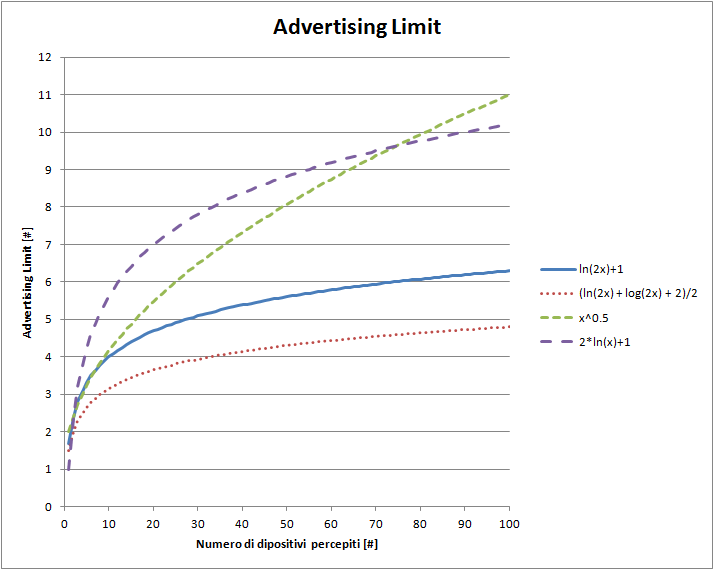
\includegraphics[width=0.9\linewidth]{Images/grafici_usati/AL_curve_no_arr}
	\caption[Curve dell'AL (continuo)]{Curve di Advertising Limit.}
	\label{fig:AL_curve_no_arr}
\end{figure}
Abbiamo riportato su grafico le funzioni appena elencate, nella \myFig{fig:AL_curve_no_arr}. Come si può notare anche dai grafici, le funzioni analizzate hanno diversi andamenti e crescono con rapidità diverse. L'\MyEq{eq:al_01} è stata la prima funzione studiata, in quanto di base ha le caratteristiche che cercavamo; un andamento reattivo per valori bassi di nodi e un comportamento crescente ma molto più limitato al crescere del numero di nodi. L'\MyEq{eq:al_02} è la media tra due funzioni logaritmiche e si è rivelata essere abbastanza conservativa. Le Equazioni \eqref{eq:al_03} e \eqref{eq:al_04} invece sono due funzioni molto simili come andamento ed entrambe molto permissive, con una crescita abbastanza rapida e costante. La funzione che abbiamo scelto di implementare nell'algoritmo è la funzione di \MyEq{eq:al_01}:
\begin{equation}
	AL=\ln \left( 2\textit{x}\right) + 1 \nonumber
\end{equation}
L'idea generale nel modellare questo parametro è stata quella di cercare di dare reattività nell'adattamento al crescere del numero di nodi percepiti, quando i nodi percepiti sono pochi. La rapidità di crescita per valori piccoli di numero di nodi, è per poter dare ai  dispositivi un limite sufficientemente ridondante che possa coprire gli eventuali nodi che con poca batteria parteciperanno poco, o nulla, alla diffusione dell'informazione e inoltre un'alto \acs{AL} con pochi nodi, aiuta a coprire problemi di diffusione relativo alle poche connessioni tra i nodi. Più il numero di nodi cresce più la necessità di questa copertura diminuisce, rendendo sufficiente una crescita dell'\acs{AL} più lenta; questo perché vi sono molti più nodi che possono coprire le eventuali mancanze e queste coperture si distribuiscono tra tutti i nodi. In \myFig{fig:AL_curve_arr} abbiamo riportato su grafico l'arrotondamento per eccesso delle funzioni analizzate riportate nel grafico in \myFig{fig:AL_curve_no_arr}, per lo stesso motivo esposto per il \acs{DF}. La versione con arrotondamento è stata implementata nell'algoritmo.

\begin{figure}[t]
	\centering
	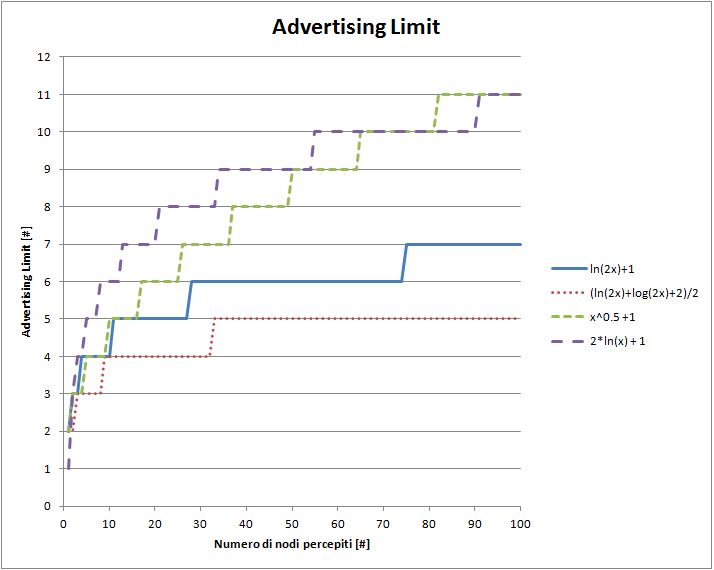
\includegraphics[width=0.9\linewidth]{Images/grafici_usati/AL_curve_arr}
	\caption[Curve dell'AL (arrotondato)]{Curve di Advertising Limit, arrotondate per eccesso.}
	\label{fig:AL_curve_arr}
\end{figure}
